For eccentric orbits, there are two primary additional physical or computational effects to consider. One is the need for a way to describe relativistic eccentric orbits. The second is that in the presence of a source, it is necessary for the particle to be at an element boundary due to discontinuities at the location of the source because the singular source is not precisely regularlized by the Detweiler-Whiting singular field. To keep the particle at an element boundary for all times by keeping the computational coordinate fixed, it is necessary to add a time dependent coordinate transformation region between tortoise layers in the middle of the computational grid~\cite{time_dependent_coordinate_transform}. In this section, I describe Peter Diener's Fortran code, using Niels Warburton's exact initial conditions for l-modes 0 through 5, and Barry Wardell's effective source, which I have run to produce eccentric orbit output. 

\section{Orbital parameters}

The eccentricity of an eccentric orbit is defined such that the turning points are defined to be $r_{periastron}=\frac{pM}{1+e}$ and $r_{apastron}=\frac{pM}{1-e}$, where $p$ is the semilatus rectum. Eccentric orbits in general relativity precess. In the coordinates of Refernce~\cite{pound_poisson}, $\chi$ is a parameter that runs from $0$ to $2\pi$ in one radial cycle (as opposed to $\phi$, which runs from $0$ to $2\pi$ in one angular cycle). The orbital parameters of an eccentric orbit in a Schwarzschild space-time are derived from General Relativity to be 
\begin{equation}
  E^2=\frac{(p-2-2e)(p-2+2e)}{p(p-3-e^2)}
\end{equation}
\begin{equation}
  L^2=\frac{p^2M^2}{p-3-e^2}
\end{equation}
For an eccentric orbit, $\chi$ and $\phi$ are evolved using a fourth order Runga Kutta integration using derivatives of $r$, $\chi$, $\phi$, and $t$, provided in Reference~\cite{pound_poisson}. For a self consistent evolving orbit with the back-reaction effect of the self-force, see future work in Chapter~\ref{futurework}. 


\section{Time dependent coordinate transformation}

In the case of an eccentric orbit, it is necessary to ensure that the particle always remains at an element boundary for all time. We use a time dependent coordinate transformation to keep the particle fixed at a specific coordinate location while the coordinates in its immediate neighborhood evolve. This simulates a particle on an eccentric orbit and produces the same self-force and the same scalar waves at scri plus. The necessary time dependent coordinate transformation can be found in Reference~\cite{time_dependent_coordinate_transformation}. It transforms from tortoise coordinates, $x$, to time dependent coordinates, $xi$. The location of the particle $x_p(t)$, varies in tortoise coordinates but is fixed in time dependent coordinates ($\xi_p$). $a$ and $b$ are the boundaries of the time dependent region, in computational coordinates. 
\begin{equation}
  x=a+\frac{x_p-a}{x_p(t)-a}(\xi-a)+\frac{(b-x_p(t))(\xi_p-a)-(x_p(t)-a)(b-\xi_p)}{(\xi_p-a)(b-\xi_p)(b-a)}(\xi-a)(\xi-\xi_p)
\end{equation}
I have used Mathematica to confirm the time dependent coordinate wave equation used in Peter Diener's Fortran scalar self-force code. Its time and radial components are
\begin{eqnarray}
\frac{d^2\psi}{dt^2}=&\left(\frac{dx}{d\xi}\right)^-3\left[\frac{d^2x}{d\xi^2}-\frac{d^2x}{d\xi^2}\left(\frac{dx}{dt}\right)^2-2\frac{d^2x}{d\xi dt}\frac{dx}{d\xi}-\left(\frac{d^2x}{dt^2}\right)^2\right]\frac{d\psi}{d\xi}\nonumber\\
&+\left[-1+\left(\frac{dx}{dt}\right)^2\right]\left(\frac{dx}{d\xi}\right)^{-2}\frac{d^2\psi}{d\xi^2}\nonumber\\
&-2\frac{dx}{dt}\left(\frac{dx}{d\xi}\right)^{-1}\frac{d^2\psi}{d\xi dt}
\end{eqnarray}

It is necessary to invert the time dependent transformation subtract the principle part of the singular field from the principle part of the state vector to obtain in-going fluxes at elements just outside the world tube. Similarly, to obtain in-going fluxes inside the world tube, we must transform to time dependent coordinates and subtract the singular field from the scalar field. For outgoing fluxes, addition and subtraction are reversed. 


\section{Orbits}

I have computed several orbits of the system for $p=9.9$, $e=0.1$. Figure~\ref{rorb} shows the radial coordinate in Schwarzschild coordinates as a function of time. Figure~\ref{phiorb} depicts the physical path of the orbit, including precession. Figure~\ref{precession} demonstrates why precession must exist. The periods of the angular variable $\phi$ and the parameter that governs the rate of radial evolution, $\chi$, are not synchronized.

\begin{figure}
  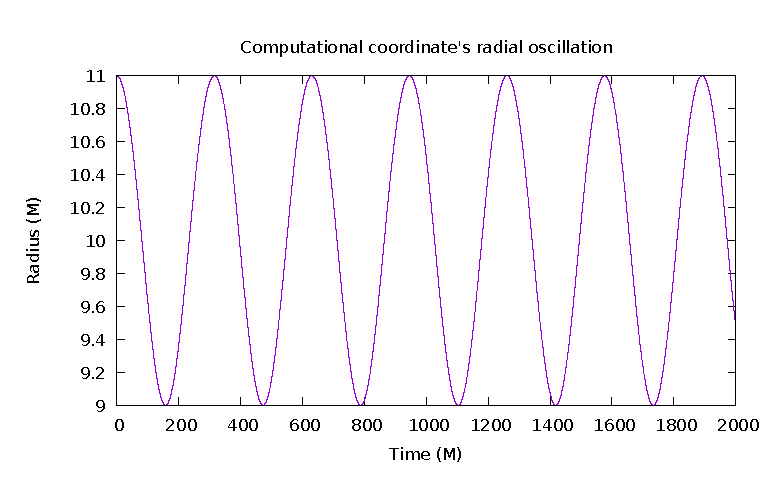
\includegraphics{orbit}
  \caption{Schwarzschild r as a function of time over several orbits. $p=9.9$, $e=0.1$}
  \label{rorb}
\end{figure}


\begin{figure}
  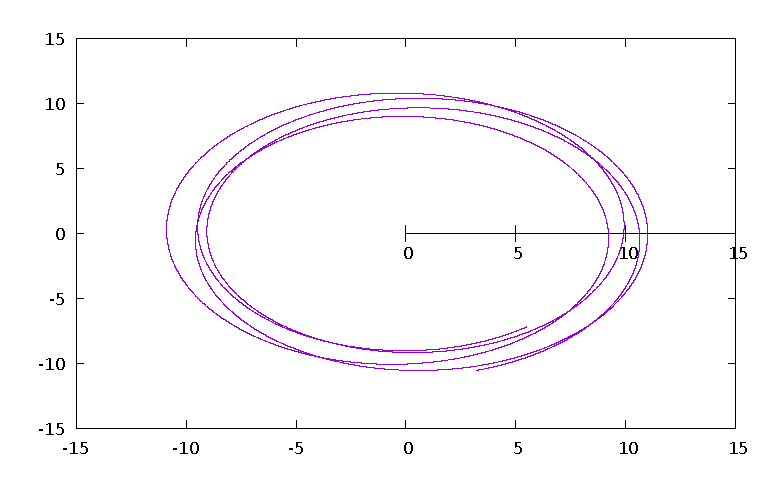
\includegraphics{orbitevolvedg44p99e01}
  \caption{The orbit as it physically would exist, using Schwarzschild $\phi$ as the polar coordinate angle. The orbit precesses but does not inspiral since there is no generic evolution. Shown for $p=9.9$ and $e=0.1$}
  \label{phiorb}
\end{figure}


\begin{figure}
  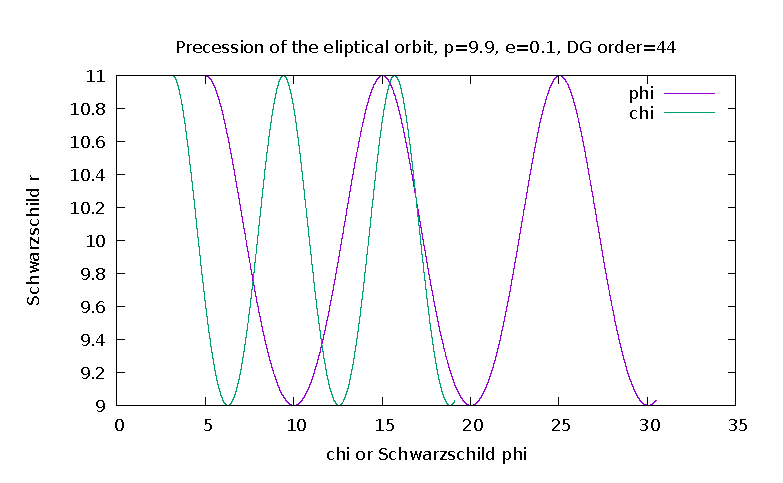
\includegraphics{precessiondg44p99e01}
  \caption{Precession of the eccentric orbit is demonstrated due to the inequality in the period of the angular variables $\chi$, which represents the period of the radial oscillations, and $\phi$, which represents the period of the angular oscillations. $p=9.9$, $e=0.1$}
  \label{precession}
\end{figure}

\section{Self force output}

The radial self-force is defined as $q\nabla^\alpha\Psi^{R}$~\cite{wardell_vega_thornburg_diener}. To compute this self force, it is necessary to sum over all l and m modes. In principle it is necessary to sum to $l=\infty$. Figures~\ref{rsf},~\ref{tsf}, and~\ref{phisf} are computed by displaying the first several individual l modes from this partial mode sum, summed over m. 


\begin{figure}
  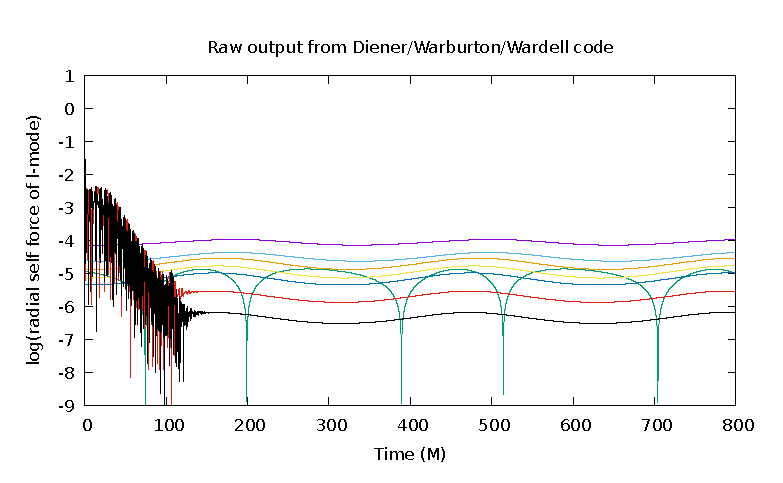
\includegraphics{rawRadialSelForceModes}
  \caption{Raw output of Diener, Warburton, and Wardell code for DG order 44. Radial self force. The first several l-modes are displayed. For modes 0 through 5, Niels Warburton's frequency domain initial conditions are used to avoid transients. For modes 6 and 7, transients converge exponentially to an oscillating waveform that has a lower amplitude for higher modes.}
  \label{rsf}
\end{figure}

\begin{figure}
  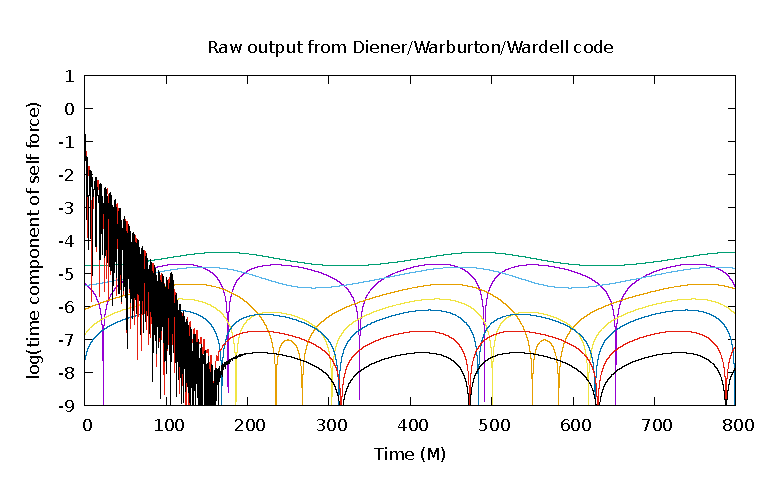
\includegraphics{rawTimeSelfForceModes}
  \caption{Raw output of Diener, Warburton, and Wardell code for DG order 44. Time component of the self force. The time component of the self force shares a similar behavior to the radial component with the self force.}
  \label{tsf}
\end{figure}

\begin{figure}
  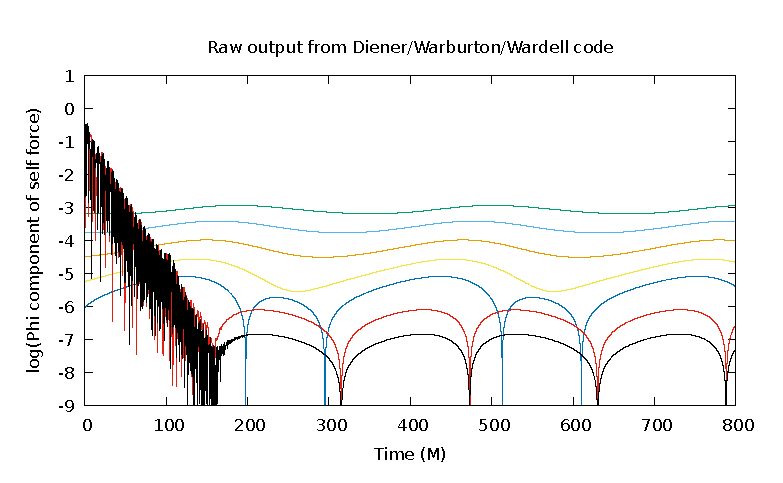
\includegraphics{rawPhiSelfForceModes}
  \caption{Raw output of Diener, Warburton, and Wardell code for DG order 44. Phi component of the self force. The phi compoent again shows this convergent behavior and the lack of transients from in the initial data from the frequency domain simulation.}
  \label{phisf}
\end{figure}

